\cotefile{36}
\scanpage{19}
\mspage{\handwritten{10}}

\deleted{\unsure{card(x}}
\[
\operatorname{card}(Y_t\handwritten{(k')}\deleted{\unsure{(t))|t))}}) \equiv a \quad \bmod p\,,
\]
où $Y_t$ est la section de $X_{k\handwritten{'}\deleted{\unsure{(t)}}}$ par l'hypersurface de $P^r_{k\handwritten{'}\deleted{(t)}}$ définie par $t$.

En effet, Deligne a vérifié, à l'aide de la formule de Verdier-Lefschetz, que pour un schéma propre $Y$ sur un corps fini, la somme alternée des traces \deleted{est donc} des frobenius\inserted{géométriques} opérant sur $H^i(Y,\underline{O}_Y)$ est \deleted{\unsure{congru|confru}} égal au nombre des points rationnels de $Y$ mod $p$. D'autre part, quitte à restreindre $U$, nous pouvons supposer que,
\[
f:\underline{Y}\handwritten{\longrightarrow} S_d
\]
étant le morphisme qu'on devine à fibres les $Y_s$ $(s\handwritten{\in}S_d)$, que \inserted{\handwritten{$f$ est plat, et que}} la formation des $R^if_*(\underline{O}_{\underline{Y}})$ commute au changement de base au dessus de $U$, \deleted{et} que les $R^if_*(\underline{O}_Y)$ sont localement libres sur $U$, enfin que $V$ est la fibre \deleted{d'un} générique d'un sous-fibré $\underline{V}$ de $R^{n-1}f_*(\underline{O}_Y)/\underline{O}_{S_d}\unsure{\otimes|\mathbin{\mathrm{x}}}H^{n-1}(X,\underline{O}_X)$, stable par frobenius, et sur lequel frobenius soit semi-simple (i.e. un épimorphisme $\underline{V}^{(p)}\handwritten{\longrightarrow}\underline{V}$). Alors la représentation du groupe fondamental du point générique $s$ de $S_d$ envisagée dans 7.1 provient d'une représentation du groupe fondamental \deleted{de} \handwritten{$\pi$} de $U$, \deleted{\illegible{1} Quitte à restreindre $U$, on peut supposer également que la partie semi-simple des fibres génériques de tous les $R^if\,(\underline{O}_{\underline{Y}})$ (pas seulement pour $i=n-1$) provient d'un sous-Module localement facteur direct, stable par frobenius, sur lequel frobenius soit semi-simple.} D'autre part, quitte à prendre $d_o$ assez grand dans 7.1, on peut supposer que \deleted{pour} $H^i(X,\underline{O}_X(-d))=0$ pour tout $i\handwritten{<}n$ et tout $d\handwritten{\geq}d_o$ (c'est ici qu'intervient l'hypothèse $X$ Cohen-Macaulay sur $X$), de sorte que pour toute section $Y_s$ de $X$ de degré $d\handwritten{\geq}d_o$ et de dimension $n-1$, l'homomorphisme $H^i(X_s,\underline{\mathbb{O}}_{X_{\handwritten{s}}})\handwritten{\longrightarrow}H^i(\unsure{\deleted{U}Y|\mathbb{Y}|W}_s,\underline{O}_{Y_s})$ sera un isomorphisme pour $i\leq n-2$, \inserted{\handwritten{un monomorphisme pour $i=n-1$.}} On voit alors que la formule de Lefschetz-Verdier donne, pour \deleted{le}\handwritten{le} point \deleted{fermé} $t$ de $U\handwritten{(k')}$, que le nombre des points \unsure{rationnels|rationelns} sur $k\handwritten{'}\deleted{(t)}$ de $Y_t$ \handwritten{satisfait}
% archive sheet number: 18
\scanpage{20}
\mspage{\handwritten{11}}
\[
\operatorname{card}Y_t(k')\equiv c_t+(-1)^{n-1}\operatorname{Tr}f_t\,,
\]
où \deleted{\unsure{x}}
\[
c_t=\handwritten{\sum_{0\leq i\leq n-1}(-1)^i}\operatorname{Trace}\text{ de }\operatorname{Frob}_{k'}\text{ opérant sur }H^i(X,\underline{O}_X)\,,
\]
et où $f_t$ est l'élément du groupe \inserted{\handwritten{quotient}} $G_o=\operatorname{Aut}_{\underline{F}_p}(V_o)$ de \handwritten{$\pi$}, \deleted{\unsure{qui est}} image de l'\unsure{\deleted{é}E|É|E}lément de frobenius de \handwritten{$\pi$} associé au point \deleted{fermé} $t\handwritten{\in}U(k')$. Quitte à passer à\inserted{remplacer d'abord $k$ par} une extension finie, \deleted{\unsure{de k}} de sorte que \deleted{\unsure{les valeurs}} $\operatorname{\unsure{\deleted{f}F|f}rob}_k$ opérant sur les $H^i(X,\underline{O}_X)$ soit à valeurs propres toutes égales à 0 ou 1, on peut supposer que $c_t$ est indépendant de $t$, \inserted{soit $c$.} Il résulte alors de 7.1 qu'il existe un élément $f$ de $G_o$ tel que $c+(-1)^{n-1}\operatorname{Tr}f\unsure{\equiv|=\deleted{x}}a\bmod p$, et il suffit donc de choisir un $t\handwritten{\in}U$ (considéré comme élément de $U(k(t))$ de telle façon que $f_t=f$. Mais ceci est possible en vertu du théorème de \rlap{\handwritten{\v{\phantom{C}}}}Cebotâref.

\margin{\figure{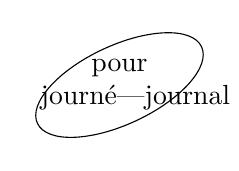
\begin{tikzpicture}\draw[rotate=25] (0,0) ellipse (1.15cm and 0.5cm);\node[text width=2cm,align=center] at (0,0) {\handwritten{pour \unsure{journé|journal}}};\end{tikzpicture}}}
\uline{Corollaire} 7.3. \inserted{(Si $n$ pair\inserted{\handwritten{$\geq4$}}, $X$ lisse).} On peut trouver un ouvert $U'$ \inserted{\handwritten{(\unsure{variété|ouvert} de la grassmannienne des droites)\deleted{de}}} de $S_d$, tel que pour toute droite \inserted{\handwritten{$D\in U'(k')$}} de $\handwritten{(}S_d\handwritten{)_{k'}}$ \deleted{qui rencontre \unsure{un|U}\handwritten{\unsure{\varnothing|k}} et qui définit}\inserted{\handwritten{$D$ est}} un pinceau de Lefschetz sur $X_{\handwritten{k'}}$, si $t$ désigne le point générique de cette droite, le motif $E(Y_t)$ des \deleted{\unsure{s}}cycles évanescents sur $Y_t$ \deleted{\unsure{soit de}} ne soit pas de niveau 1 (donc ne contienne pas de sous-motif $\handwritten{\ne}0$ de niveau 1, pas même sur une extension de $k(t)$, d'après le résultat de simplicité rappelé au n°6).
\margin{\handwritten{($k'$ une ext. qqle. de $k$)}}

On prend $U$ comme dans la démonstration de 7.2, \inserted{\handwritten{et tel que les $Y_s$ $(s\in U)$ soient lisses.}} On peut (grâce au fait qu'un motif de niveau $\handwritten{\leq}\deleted{\unsure{\leq}}1$ se spécialise en un motif de niveau $\handwritten{\leq}1$, comme on a signalé au n°6 comme conséquence du critère de Ogg-Néron-Chafarévitch) supposer que $k$ est fini, et \unsure{il|on} \deleted{\unsure{est ramené à prouver que}} suffit de prouver que l'on peut trouver un point fermé $s$ de $D\handwritten{\cap U}$ tel que les valeurs propres de Frobenius opérant sur $E^{n-1}(Y_s,\underline{Q}_{\handwritten{\unsure{\ell|l}}})$ ($\handwritten{\ell}$ un nombre premier fixé $\handwritten{\ne\ell}$) ne soient pas toutes divisibles par $p$. Or le nombre de points de $Y_t$ est égal à la somme alternée des traces de frobenius opérant sur les \deleted{\handwritten{\unsure{$H$}}}
\margin{\figure{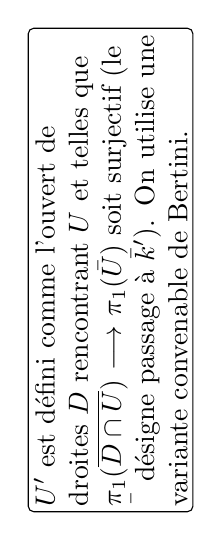
\begin{tikzpicture}\node[draw,rounded corners=2pt,rotate=90,text width=6cm,align=left,inner sep=2pt] {\handwritten{$U'$ est défini comme \unsure{l'ouvert} de droites \inserted{$D$} rencontrant $U$ et telles que $\pi_1(\overline{D\cap U})\longrightarrow\pi_1(\bar U)$ soit surjectif (le $\bar{\phantom{k}}$ désigne passage à $\bar{k}'$). On utilise une \uline{variante} \unsure{convenable} de Bertini.}};\end{tikzpicture}}}
% archive sheet number: 19
\scanpage{21}
\mspage{\handwritten{12}}
$H^i(Y_{\handwritten{\bar t}},\underline{Q}_{\handwritten{\unsure{\ell|l}}})$, qui peut s'écrire, grâce aux théorè\unsure{\deleted{n}m|m}e\unsure{\deleted{s}|s} de Lefschetz
\margin{\handwritten{faible \unsure{et}}}
\[
\begin{aligned}
&\deleted{2}\handwritten{\sum_{0\leq i\leq n-2}}\inserted{\handwritten{(-1)^i}}\operatorname{Trace}\operatorname{Frob}_{H^i(X_{\bar t},Q_{\handwritten{\ell}})}\deleted{(-1)^{\unsure{i|-1}}}\inserted{\handwritten{(1+q^{\unsure{2n-1-i|2n-2-i}})}}\deleted{+(-1)^{n-1}}\handwritten{+}\inserted{\handwritten{(-1)^{\unsure{n-1}}}}\operatorname{Trace}\operatorname{Frob}_{H^{n-1}(X_{\bar t}}\\
% The supplied scan cuts off the first line at the right edge after X and its subscript.
&\deleted{\unsure{+(-1)}}\handwritten{+(-1)^{\unsure{n-1}}}\operatorname{Trace}\operatorname{Frob}_{{\unsure{\mathbb{E}|E}}^{n-1}(Y_s,\underline{Q}_{\handwritten{\ell}})}\,,
\end{aligned}
\]
\margin{\handwritten{$q=\operatorname{card}k(s)$}}
où tous les frobenius sont relatifs au corps de base $k(\unsure{s|t})$. Ici encore, quitte à remplacer $k\deleted{\unsure{x}}$ par une extension finie, on peut supposer que les valeurs propres de\handwritten{s} frobenius (relatifs à $k$) opérant sur les $H^i(X_{\bar k},\underline{Q}_{\handwritten{\ell}})$ \inserted{\handwritten{$(0\leq i\leq n-2)$}} soit égales à 0 ou 1 mod $p$ \inserted{\handwritten{(en tant qu'entiers algébriques)}}, de sorte que mod $p$ \deleted{les} la contribution des termes de la première ligne soit indépendante de choix de $s$, \inserted{soit $c$.} Donc si les valeurs propres de frobenius opérant sur les $E^{n-1}(Y_s,\underline{Q}_{\handwritten{\ell}})$ \deleted{\unsure{étaient}}\inserted{sont} toutes divisibles par $p$, on en conclut\deleted{\unsure{alors que pour} tout point fermé} que $\operatorname{card}Y_{s}(k(t))\equiv c\quad\bmod p$, et la même relation serait également valable, pour la même raison, si on remplace $k(t)$ par une extension finie $k'$ quelconque. \deleted{Or on peut d'après} Il suffit donc de voir qu'on peut trouver toujours un point \deleted{fermé} $s$ de $D\handwritten{\cap}U$ \deleted{tel que le}\inserted{dans une}\deleted{nombre}\inserted{extension finie $k'$ de $k$, tel que} $\operatorname{card}Y_s(k\handwritten{'}\deleted{(s)})\deleted{\unsure{x}}$ soit congru mod $p$ à un élément donné de $\underline{F}_p$ (\unsure{qu'on} choisi\unsure{\deleted{r}t|\deleted{t}r}a alors $\handwritten{\ne}c$). Or c'est ce que montre essentiellement 7.2, à cela près qu'on n'a pas été assez précis dans l'énoncé de ce corollaire puisqu'on peut imposer à $s$ de provenir de $D\handwritten{\cap}U\,(k')$, où $D$ est une droite donnée \inserted{\handwritten{$\in U'(k')$ \deleted{\unsure{convenable}}}} rencontrant $U$. Ce raffinement est contenu dans la démonstration de 7.2, compte tenu du fait que par $\unsure{\mathbb{B}|B}$ertini, le groupe \unsure{fondamental}\deleted{\unsure{s}} de $\handwritten{(}D\handwritten{\cap}U\handwritten{)_{k'}}$ s'envoie \uline{sur} celui de $U$, donc s'envoie \uline{sur} $G_o$.
% archive sheet number: 20
\scanpage{22}
\mspage{\handwritten{13}}
\uline{Remarques} 7.4. a) Remords à 7.3. Inutile de supposer $n$ pair et $n\handwritten{\geq}4$, en énonçant la conclusion sous la forme: le niveau de $E^{n-1}(Y_t)$ est égal à $n-1$ $(n\handwritten{\geq}1)$. On n'a pas besoin en effet d'un critère de Ogg-Néron-Chafarévitch ici, car il suffit de savoir que \uline{si} $E^{n-1}(Y_t)$ est de niveau $\handwritten{<}n-1$, i.e. s'il existe sur \deleted{$k(t)$} $\bar{k}'$ $(k'=k(t))$ un cycle sur un produit $Z\mathbin{\mathrm{x}}Y_{\overline{k'}}$ définissant un \deleted{iso}\inserted{épi}morphisme $H^{n-3}(Z,\underline{Q}_{\handwritten{\unsure{\ell|l}}})(-1)\handwritten{\longrightarrow}H^{n-1}(Y_{\bar{k}'},\underline{Q}_{\handwritten{\ell}})\handwritten{\unsure{-|\to}}E(Y_{\bar{k}'})$ \deleted{\unsure{alors quitte à passer pour}} alors pour tout $s\handwritten{\in}D$ assez voisin de $t$, la même conclusion est vraie pour $E(Y_s)$, comme on constate aussitôt; de sorte que, si $s$ est à corps résiduel fini, les valeurs propres du frobenius opérant sur $E^{n-1}(Y_{\bar{s}})$ sont divisibles par \deleted{la} $\operatorname{card}k(t)$ et a fortiori par $p$. Or cela est impossible si $D$ estchoisieassez générale, de façon qu'on puisse appliquer Bertini. D'autre part, même si $n$ est impair i.e. $n-1$ pair, de sorte qu'on ne peut plus affirmer que la \deleted{\unsure{restri}}\deleted{b) Bien entendu, ce n'est que par commodité de langage qu'on a} représentation de monodromie sur $E^{n-1}(Y_{\bar t})$ \unsure{\deleted{e}r|r}este simple quand on la restreint à un sous-groupe ouvert quelconque de $G=\operatorname{Gal}(\overline{k(t)}/k(t))$, il sera vrai néanmoins qu'aucun sous-motif non nul de $E^{n-1}(Y_{\bar t})$ n'est de niveau $\handwritten{<}n-1$. En effet, le plus grand sous-motif \inserted{de niveaù $n-1$} de $E^{n-1}(Y_{\bar t})$ \deleted{qui est de niveau $n-1$} définit un sous-espace de $E^{n-1}(Y_{\bar t},\underline{Q}_{\handwritten{\ell}})$, qui\deleted{\unsure{n}} est évidemment stable sous le groupe de Galois.

b) Nous avons utilisé le langage des motifs par pure commodité pour l'énoncé de 7.3. Comme ce langage n'est pas justifié à l'heure actuelle, il est préférable, pour le moment, de l'énoncer en termes de la filtration par le niveau sur la cohomologie \handwritten{$\ell$}-adique, en définissant celle-ci en conformité avec a) (La définition plus naturelle en termes de la filtration de l'espace $Y_{\bar t}$ par les supports devrait être équivalente, mais ceci utiliserait la résolution des singularités). Ceci dit, l'énoncé 7.3 (sous la forme plus générale a) ci-dessus) est démontré sans aucune conjecture (pas même Lefschetz vache pour $X$ \ldots).
% archive sheet number: 21
\scanpage{23}
\mspage{\handwritten{14}}
\uline{Démonstration de} 7.1. Nous prendrons \deleted{pour} $d_o$ \deleted{le plus petit entier} \deleted{\unsure{qui}} tel que l'on ait \handwritten{(entre autres)}
\[
\deleted{\handwritten{d}_o\unsure{\geq|-}n+1}\qquad H^i(X,\underline{O}_X(-d))=0\quad\text{pour tout }d\handwritten{\geq}d_o,\ i<n.
\tag*{\handwritten{(*)}}
\]
Désignons par $U$ l'ouvert de $S_d$ formé des $\unsure{s|t}\handwritten{\in}S_d$ tels que $\dim Y_s=n-1$, qui est aussi le plus grand ouvert tel que $\underline{Y}\handwritten{\longrightarrow}S_d$ soit plat au dessus de $U$. Comme on a signalé, le choix de $d_o$ implique que pour tout $s\handwritten{\in}U(k')$, les homomorphismes
\[
H^i(X_{k'},\underline{O}_{X_{k'}})\handwritten{\longrightarrow}H^i(Y_s,\underline{O}_{Y_s})
\tag*{\handwritten{(**)}}
\]
sont des isomorphismes pour $i\handwritten{\unsure{\leq|<}}n-2$, un monomorphisme pour $i=n-1$. Ceci implique, par EGA III 7, que les\deleted{R} $R^if_*(\underline{O}_{\underline{Y}})$ sont plats sur $U$ et y commutent à l'extension de la base, en particulier au passage aux fibres. On fera attention que même si $X$ est lisse et géom. connexe, nous serons obligés de façon essentielle de travailler avec des points $s\handwritten{\in}U$ pour lesquels $Y_s$ n\deleted{e}'est pas \unsure{irréductible|irréductiible} et a fortiori non lisse. Ce ne sera qu\deleted{e}\handwritten{'} une fois que 7.1 est démontré qu'on pourra en tirer des conclusions \inserted{diophantiennes} sur des points femmés dans un ouvert arbitrairement petit de $S_d$ comme dans 7.2, puis les appliquer comme dans 7.3.

Bien entendu, il suffit de prouver 7.1 après extension arbitraire du corps de base $k$, ce qui nous permettrait en particulier de supposer $k$ algébriquement clos; et la conclusion se renforce \inserted{dans le cas général} automatiquement, en remplaçant le groupe de Galois $G$ envisagé par le sous-groupe image du groupe de Galois provenant de la situation géométrique où $k$ est remplacé par $\bar{k}$. Mais pour ppouver 7.1, nous procèderons \inserted{\handwritten{au contraire}} par voie arithmétique, en notant qu'on peut se réduire au cas où $k$ est fini. Cette réduction se fait \handwritten{de} la façon habituelle, et n'offre pas de difficultés. \deleted{Quitte} On peut alors considérer les frobenius ``géométriques'' opérant sur les $H^i(X,\underline{O}_X)$; si $k$ a $q=p^m$ éléments, c\deleted{'}\handwritten{e} \deleted{est}\inserted{\handwritten{sont}} l\deleted{a}\handwritten{es} puissance\handwritten{s} m-ème\handwritten{s} d\deleted{u}\handwritten{es} frobenius
% archive sheet number: 22
\scanpage{24}
\mspage{\handwritten{15}}
$p$-linéaire\handwritten{s} opérant sur les $H^i(X,\underline{O}_X)$. Quitte à remplacer $k$ par une extension finie, on peut supposer que toutes les valeurs propres desdits frobenius sont égales à 0 ou 1. Soit $c$ la somme alternée \deleted{\unsure{des valeurs} valeurs des du nombre} des rangs semi-simples des $H^i(X,\underline{O}_X)$ pour $0\handwritten{\leq}i\handwritten{\leq}n-1$. Alors pour toute extension finie $k'$ de $k$, la somme alternée des traces de $\operatorname{frob}_{k'}$ opérant sur les $H^i(X_{k'},\underline{O}_{X_{k'}})$ est \deleted{alors}\deleted{\handwritten{\unsure{encore}}} égale à $c$. En vertu de Lefschetz-Verdier Deligne, et des isomorphismes (**), on conclut que pour tout point $s\handwritten{\in}U(k')$, on a
\[
\operatorname{card}Y_{\unsure{s|t}}(k')\equiv c+(-1)^{n-1}\operatorname{Tr}f_s\,,
\tag*{\deleted{\unsure{***|xxx}}}
\]
où $f_s\handwritten{\in}G_o$ est \deleted{l'image de l'élément de Frobenius de} le frobenius relatif à $k'$ opérant sur $E_o(Y_s)$. Ceci posé, 7.1 est une conséquence des deux lemmes suivants;

\margin{\figure{\begin{tikzpicture}[x=1cm,y=1cm]\node at (0,0.3) {\handwritten{!}};\draw (0.45,-0.8)--(0.52,1.5);\end{tikzpicture}}}
\uline{Lemme} 7.5. Pour tout $s\handwritten{\in}U$, il existe un élément $f\handwritten{\in}G_o$ \inserted{\handwritten{et $V'_o\subset V_o$ \unsure{stable} par $f$}} tel que le polynôme caractéristique de $f$ opérant sur \figure{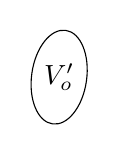
\begin{tikzpicture}\node at (0,0) {$V_o^{\handwritten{\prime}}$};\draw[rotate=-8] (0,0) ellipse (0.35cm and 0.6cm);\end{tikzpicture}} soit égal à celui de $f_s$, et en particulier tel que $f\handwritten{|_{V'_o}}$ et $f_s$ aient même trace.

\uline{Lemme} 7.6. Pour tout entier $N\handwritten{\geq}0$, il existe un entier $d^{\handwritten{\prime}}_o$ \inserted{\handwritten{$>0$}} tel que pour tout entier $d\handwritten{\geq}d'_o$, il existe une extension finie $k'$ de $k$ et un point $s\handwritten{\in}U_d(k')$ tel que $\operatorname{card}(Y_s)=N$. (Marche dès que $X$ est un sous-schéma fermé de $P^r_k$ de dimension $n\handwritten{\geq}1$.)

\uline{Démonstration de} 7.6. \inserted{\handwritten{On peut supposer $X$ réduit.}} Soit $r$ la \inserted{somme des} degrés des composantes irréductibles réduites de $X$ qui sont de\deleted{d} dimension $n$, et soit $d_1$ un entier tel que
\[
N\handwritten{\geq}rd_1^n\,.
\]
Quitte à passer à une extension finie de $k$, on peut supposer \deleted{que chaque composante irréductible $X_i$ de $X$ \inserted{est géom. irréductible et} contient un point rationnel sur $k$ qui\unsure{\,$x_i$} n'appartient à aucune et que} les composantes irréductibles $X_i$ de $X$ géométriquement irréductibles, que tout $X_i$ contient un $x_i\handwritten{\in}X_i(k)$, et qu'il existe $n$ formes $\handwritten{\phi}_o,\ldots,\handwritten{\phi}_{n-1}$ de degré $d_1$ sur $P^r_k$,
% archive sheet number: 23
\scanpage{25}
\mspage{\handwritten{16}}
définissant des hypersurfaces $H_o,..H_{n-1}$ telles que $X\handwritten{\cap}H_o\handwritten{\cap}..\handwritten{\cap}H_{n-1}=Z$ soit un schéma fini \inserted{\handwritten{étale}} sur $k$, de degré $rd_1^n$, dont tous\deleted{\unsure{es}} les points sont rationnels sur $k$\inserted{et distinct des $x_i$.}. Quitte à augmenter $k$ et $d_1$, on peut supposer qu'il existe une forme $\handwritten{\phi}_n$ de même degré $d_1$, définissant $H_n$, tel\handwritten{\unsure{le|l|e}} que $H_n\handwritten{\cap}Z$ soit de cardinal $N$. Pour tout entier $d_2\handwritten{\geq}n+1$, on sait qu'il existe une forme \handwritten{$\underline{\phi}$} à $n+1$ variables \deleted{telle que} définie sur $k$, de degré $d_2$, \deleted{telle que} n'ayant pas de zéro non trivial sur $k$. Alors
\[
\handwritten{\phi}=\handwritten{\underline{\phi}}\,(\handwritten{\phi}_o,\ldots,\handwritten{\phi}_n)
\]
est une forme de degré $d_2d_1$ sur $P^r_k$, telle que $(H_{\handwritten{\phi}}\handwritten{\cap}X)(k)=(H_n\handwritten{\cap}Z)(k)$ soit de cardinal $N$. De plus, comme cet ensemble ne contient pas les $x_i$, \handwritten{$\phi$} définit bien un point de $U_{d_1d_2}$. Lorsque $N$ est 0 ou 1\inserted{(plus généralement $N\handwritten{\leq}r$)}, on a terminé, car on peut prendre $d_1=1$, et 7.6 marche avec $d'_o=n+1$. Si on a $N>r$, on note que pour tout $d_{\handwritten{3}}\handwritten{\geq}n+1$, il existe une forme \handwritten{$\unsure{\psi|\mu}$} de degré $d_{\handwritten{3}}$ \inserted{rat/$k$} telle que $(H_{\handwritten{\psi}}\handwritten{\cap}X)(k)=\handwritten{\varnothing}$ d'après ce qu'on vient de voir, et alors la forme \handwritten{$\phi\ \psi$} est de degré \inserted{$d=$} $d_1d_2+d_{\handwritten{3}}$ et $(H_{\handwritten{\phi\psi}}\handwritten{\cap}X)(k)=Z(k)$ a comme cardinal $N$, et \handwritten{$\phi\psi$} définit encore un élément de $U_d$. On peut donc prendre alors $d'_o=d_1\handwritten{\unsure{d|\phi}}_2+(n+1)=(d_1+1)(n+1)$ (en prenant, comme il est loisible, $d_2=n+1$.

\uline{Remarques} 7.7. \handwritten{a)} On trouve ainsi une estimation assez précise de $d'_o$ de 7.6 \deleted{\unsure{(donc}} en fonction de $N$ et de $r$, donc du $d_o$ de 7.1 en fonction de $N=p-1$ et de $r$, \deleted{\unsure{lorsqu'on désire dans}} et du plus petit entier rendant valables les égalités (*). Lorsque dans la conclusion de 7.1 on se contente d'affirmer que les éléments de $G_o$ donnent lieu à au moins deux traces distinctes (ce qui suffit à conclure que $G_o$ n'est pas un $p$-groupe et a fortiori n'est pas le groupe unité, donc $\dim V\handwritten{\geq}1$ i.e. frobenius sur $V$ n'est pas nilpotent) on peut prendre \deleted{pour} simplement $d'_o=n+1$, et pour $d_o$ le plus petit entier $\handwritten{\geq}n+1$ tel que l'on ait (*). Ce choix de $d_o$ est suffisant aussi, par conséquent, pour avoir la validité des
% archive sheet number: 24
\scanpage{26}
\mspage{\handwritten{17}}
conclusions de 7.2, sous la forme \unsure{affaablie|affaiblie} qu'on peut \deleted{résoudre} satisfaire à la congruence envisagée pour au moins deux valeurs de $a$ distinctes mod. $p$, et par suite pour avoir la conclusion de 7.3 (qui n'utilise essentiellement que 7.2 sous cette forme affaiblie).

\inserted{b)} Lorsqu'on veut 7.6 avec un $N$ donné, on \deleted{peut aussi} pourra sans doute trouver souvent une meilleure majoration de $d'_o$ que $(d_1\handwritten{+}1)(n+1)$, en décomposant $N$ en $N'+N''$, en choisissant $d'_1$ et $d''_1$ de façon que $N'\handwritten{\geq}rd_1'{}^n$, $N''\handwritten{\geq}rd_2'{}^n$, et construisant une forme produit de degré \inserted{$d=$} $d'_1\unsure{d''_2|d'_2}+d''_1d''_2$ ($d'_{\unsure{2|1}},d''_2$ des entiers arbitraires $\handwritten{\geq}n+1$) dont l'ensemble des zéros communs avec $X$ rationnels sur $k$ soit la somme disjointe de deux ensembles de cardinaux respectifs $N'$ et $N''$. Quitte à choisir $d'_1$ et $d''_1$ \deleted{assez gra} premiers entre eux, on trouve \inserted{que} tout entier assez grand $d$ \inserted{se met} sous la forme envisagée.

c) On fera attention que les formes auxiliaires sans zéro non trivial utilisées dans la démonstration de 7.6 sont construites avec des formes normiques, et sont toujours décomposables géométriquement en facteurs linéaires. Ceci précise la remarque faite au début de la démonstration de 7.1 concernant la nécessité de travailler avec le gros ouvert $U_d$ tout entier.

Indiquons pour terminer la raison générale pour 7.5 :

\uline{Lemme} 7.8. Soient $S$ un schéma\inserted{\handwritten{normal}} de car. $p>0$, $\underline{V}$ un Module localement libre de type fini sur $S$ muni d'un \inserted{\handwritten{endo}}morphisme $p$-linéaire\deleted{x} $f$, $t$ un point de $s$ et $s$ une spécialisation de $t$. Considérons les représentations des groupes $G_t=\operatorname{Gal}(\overline{k(t)}/k(t))$ et $G_s=\operatorname{Gal}(\overline{k(s)}/k(s))$ dans des vectoriels de dimension finie $V_1$ resp. $V_o$ sur le corps premier $\underline{F}_p$, définis par les parti s semi-simples des fibres \deleted{de} réduites de $\underline{V}$ en $t$ resp. en $s$. Alors il existe un sous-espace $V'_o$ de $V_1$, stable par un sous-groupe ouvert $G'_t$ de $G_t$, tel \inserted{que} la représentation de l'image $G'_{t\,o}$ de $G'_t$ dans \deleted{$V'$} $\operatorname{Aut}(V'_o)$ par automorphismes de $V'_o$ soit isomorphe à celle de l'image $G_{s\,\unsure{o}}$
% Last subscript at the lower edge is partly cropped in the supplied image.
% archive sheet number: 25
\scanpage{27}
\mspage{\handwritten{18}}
de $G_s$ dans $\operatorname{Aut}V_o$ par a\deleted{t}\handwritten{u}\deleted{u}\handwritten{t}omorphismes de $V_o$, \unsure{\deleted{n}\handwritten{v}|\deleted{v}\handwritten{v}}\deleted{o}ia un isomorphisme convenable de $G'_{t\,o}$ \unsure{\deleted{e}a\deleted{t}ve\deleted{d}c|avec} $G_{s\,o}$.

La démonstration de 7.8 est par l'âne qui trotte, en se ramenant au cas $S$ \inserted{\handwritten{intègre}} hensélien de point fermé $s$, \handwritten{point générique $t$.}

\handwritten{8. Relations heuristiques entre cohomologie cristalline et le \unsure{quasi-|topo-}cristallin, et le cohomologie évanescente.}

\handwritten{(J'ai donné \unsure{notes|note} à Berthelot)}
% archive sheet number: 26
